\documentclass[14pt]{extarticle} 
\usepackage{unicode-math}
\usepackage{amsthm,graphicx,xcolor,natbib,enumitem,booktabs,tabularx}
%\usepackage[paperwidth=126mm, paperheight=96mm, top=5mm, bottom=5mm, right=5mm, left=5mm]{geometry}
\usepackage[margin=1cm]{geometry}
\pagenumbering{gobble}

\usepackage[BoldFont,SlantFont]{xeCJK}  
\xeCJKsetemboldenfactor{2}
\setCJKmainfont{cwTeX Q Yuan Medium}
%\setCJKmainfont{cwTeX Q Kai Medium}
%\setCJKmainfont{cwTeX Q Ming Medium}
%\setCJKmainfont[AutoFakeSlant=.1,AutoFakeBold=1]{cwTeX Q Kai Medium} 
%\setCJKfamilyfont{kaiv}[Vertical=RotatedGlyphs]{cwTeX Q Medium}
%\setmainfont{texgyrepagella-regular.otf}
%\setmathfont{texgyrepagella-math.otf}
\newcommand{\ds}{\displaystyle}
\newcommand{\ie}{\,\Longrightarrow\,}
\newcommand{\ifff}{\,\Longleftrightarrow\,}
\newcommand{\mi}{\mathrm{i}}
\DeclareMathOperator*{\dom}{dom}
\DeclareMathOperator*{\codom}{codom}
\DeclareMathOperator*{\ran}{ran}
\newcommand{\floor}[1]{\lfloor #1 \rfloor}
\newcommand{\ceil}[1]{\lceil #1 \rceil}

% figure --> 圖
\renewcommand{\appendixname}{附錄}
\renewcommand{\figurename}{圖}
\renewcommand{\tablename}{表}
\renewcommand{\refname}{參考文獻}

\usepackage{hyperref}
\hypersetup{
    colorlinks,
    linkcolor={red!50!black},
    citecolor={blue!60!black},
    urlcolor={blue!60!black}
    %urlcolor={blue!80!black}
}

\theoremstyle{definition}
\newtheorem*{dfn}{定義}
\newtheorem*{prp}{性質}
\newtheorem*{thm}{定理}
\newtheorem*{ex}{例}
\newtheorem*{sol}{解}
\newtheorem*{prf}{證}

%\setenumerate{label=(\roman*),itemsep=1pt,topsep=3pt}
\newcommand{\myline}{\noindent\makebox[\linewidth]{\rule{\paperwidth}{0.4pt}}}
%\newcommand{\myline}{\textcolor[RGB]{220,220,220}{\rule{\linewidth}{1pt}}}

\usepackage{tikz}
\usetikzlibrary{arrows.meta,angles,quotes}
\usepackage{pgfplots}
% axis style, ticks, etc
\pgfplotsset{every axis/.append style={
                   label style={font=\fontsize{4}{4}\selectfont},
                   tick label style={font=\fontsize{4}{4}\selectfont}  
               },
            }
\renewcommand\tabularxcolumn[1]{m{#1}}

\begin{document}
\title{\texorpdfstring{\vspace{-15mm} 內心座標公式}{內心座標公式}} 
\author{\vspace{-4em}}
\date{\vspace{-4em}}

\maketitle

\begin{thm}[內心座標公式]
  如圖,$\Delta ABC$ 中 $\overline{BC} = a$,$\overline{AC} = b$,$\overline{AB} = c$,點 $A'$、$B'$、$C'$ 分別位在 $\overline{BC}$、$\overline{AC}$、$\overline{AB}$ 上且 $\overline{AA'}$、$\overline{BB'}$、$\overline{CC'}$ 分別為角 $A$、$B$、$C$ 的平分線並相交於 $O$。若座標 $A = (x_1, y_1)$、$B = (x_2, y_2)$、$C = (x_3, y_3)$,則內心 $O$ 座標為 
\begin{align*}
  O = \frac{a}{a + b + c}\,A + \frac{b}{a + b + c}\,B + \frac{c}{a + b + c}\,C = \left(\frac{a\,x_1 + b\,x_2 + c\,x_3}{a + b + c},\,\frac{a\,y_1 + b\,y_2 + c\,y_3}{a + b + c}\right) 
\end{align*}
\begin{figure}[!htbp]
  \centering
  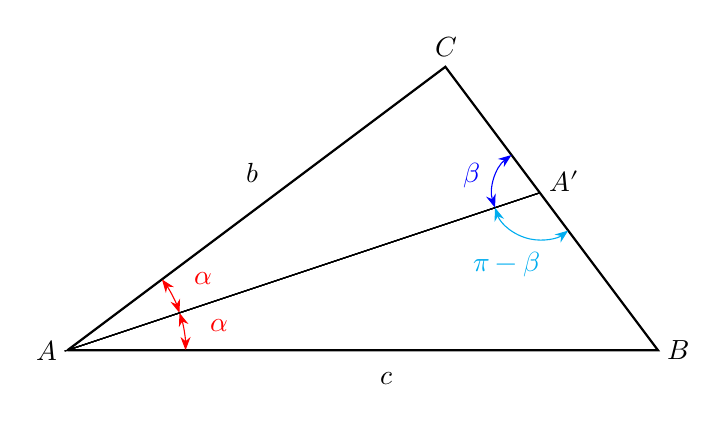
\begin{tikzpicture}[scale=1.5, >={Stealth[scale=1]}]
    \draw (0, 0) node[left] {$A$};
    \draw (5, 0) node[right] {$B$};
    \draw (16 / 5, 12 / 5) node[above] {$C$};
    \draw (4, 4 / 3 + 0.1) node[right] {$A'$};
    \draw (8 / 5 + 0.1, 6 / 5 + 0.3) node[left] {$b$};
    \draw (2.5 + 0.2, -0.1) node[below] {$c$};
    \draw[thick] (0, 0) -- (5, 0) -- (16 / 5, 12 / 5) -- (0, 0);
    \draw (0, 0) -- (4, 4 / 3);
    \draw (16 / 5, 12 / 5) coordinate (a) -- (0, 0) coordinate (b) -- (4, 4 / 3) coordinate (c) pic ["$\alpha$",red,draw,<->,angle eccentricity=1.3,angle radius=15mm] {angle = c--b--a};
    \draw (4, 4 / 3) coordinate (a) -- (0, 0) coordinate (b) -- (5, 0) coordinate (c) pic ["$\alpha$",red,draw,<->,angle eccentricity=1.3,angle radius=15mm] {angle = c--b--a};
    \draw (16 / 5, 12 / 5) coordinate (a) -- (0, 0) coordinate (b) -- (4, 4 / 3) coordinate (c) pic ["$\beta$",blue,draw,<->,angle eccentricity=1.4,angle radius=6mm,pic text options={shift={(-2pt,-1pt)}}] {angle = a--c--b};
    \draw (4, 4 / 3) coordinate (a) -- (0, 0) coordinate (b) -- (5, 0) coordinate (c) pic ["$\pi - \beta$",cyan,draw,<->,angle eccentricity=1.4,angle radius=6mm,pic text options={shift={(-5pt,-3pt)}}] {angle = b--a--c};
  \end{tikzpicture}
  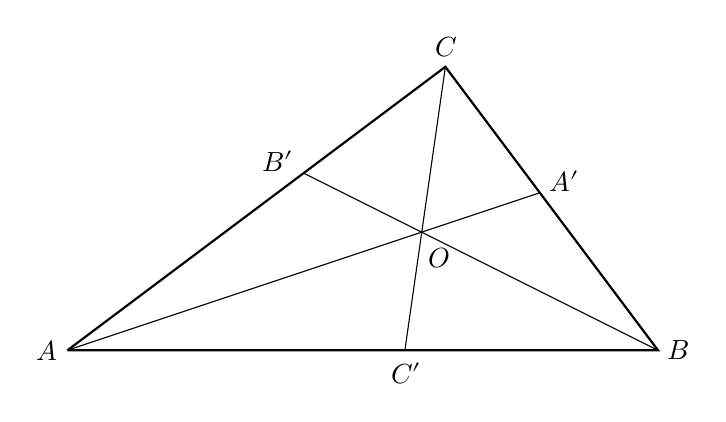
\begin{tikzpicture}[scale=1.5, >={Stealth[scale=1]}]
    \draw (0, 0) node[left] {$A$};
    \draw (5, 0) node[right] {$B$};
    \draw (16 / 5, 12 / 5) node[above] {$C$};
    \draw (20 / 7 - 0.2, -0.2) node[right] {$C'$};
    \draw (2, 3 / 2 + 0.1) node[left] {$B'$};
    \draw (4, 4 / 3 + 0.1) node[right] {$A'$};
    \draw (3 + 0.15, 1 - 0.05) node[below] {$O$};
    \draw[thick] (0, 0) -- (5, 0) -- (16 / 5, 12 / 5) -- (0, 0);
    \draw (16 / 5, 12 / 5) -- (20 / 7, 0);
    \draw (5, 0) -- (2, 3 / 2);
    \draw (0, 0) -- (4, 4 / 3);
  \end{tikzpicture}
\end{figure}
\end{thm}
  
\begin{prf}
  \begin{itemize}
    \item[]
    \item 如上圖左,首先證明若 $\ds\overline{AA'}$ 為角 $A$ 平分線,$A'$ 在 $\overline{BC}$ 上,則
      \begin{align*}
        \overline{AB}:\overline{AC} = \overline{A'B}:\overline{A'C}
      \end{align*}
      由正弦定理,在 $\Delta AA'B$ 中 $\ds\frac{\overline{A'B}}{\sin\alpha} = \frac{\overline{AB}}{\sin(\pi - \beta)} = \frac{\overline{AB}}{\sin\beta}$,在 $\Delta AA'C$ 中 $\ds\frac{\overline{A'C}}{\sin\alpha} = \frac{\overline{AC}}{\sin\beta}$;由此二式得 $\overline{AB}:\overline{AC} = \overline{A'B}:\overline{A'C}$。
    \item 反覆應用上述角平分線定理於上圖右:$\ds\overline{C'A}:\overline{C'B} = b:a$,$\ds\overline{AB} = c$,故 $\ds\overline{C'A} = \frac{b\,c}{a + b}$,又 $\ds\overline{OC'}:\overline{OC} = \overline{C'A}:\overline{CA} = \frac{b\,c}{a + b}:b = c:(a + b)$。
    \item 應用共線向量性質:若 $A$、$C'$、$B$ 依序共線且 $\overline{C'A}:\overline{C'B} = b:a$,則
      \begin{align*}
        C' = \frac{a}{a + b}\,A + \frac{b}{b + c}\,B
      \end{align*}
      又 $C'$、$O'$、$C$ 依序共線且 $\overline{OC'}:\overline{OC} = c:(a + b)$,則
      \begin{align*}
        O &= \frac{a + b}{a + b + c}\,C' + \frac{c}{a + b + c}\,C \\ 
          &= \frac{a + b}{a + b + c}\,\bigg(\frac{a}{a + b}\,A + \frac{b}{b + c}\,B\bigg) + \frac{c}{a + b + c}\,C \\ 
          &= \frac{a}{a + b + c}\,A + \frac{b}{a + b + c}\,B + \frac{c}{a + b + c}\,C
      \end{align*}
  \end{itemize}
\end{prf}

\end{document}
